\EnableTitleSlide
\section{Aufbau \& Entwicklung \\ der Anwendung}

\begin{frame}{egg}
    \begin{columns}[c]
        \column{.7\textwidth}
            \begin{itemize}
                \item \textbf{egg}: \textbf{e}-\textbf{g}raphs \textbf{g}ood (\url{https://egraphs-good.github.io/})
                \item Bibliothek in Rust zur Erstellung von E-Graphs
                \item \textbf{Paper}: Willsey u.a. 2021~\cite{2021-egg} (\url{https://doi.org/10.1145/3434304})
            \end{itemize}\hspace{2.5cm}
        \column{.3\textwidth}
            
\includegraphics[scale=1.9]{utils/egg.pdf}
    \end{columns}
\end{frame}

\begin{frame}{Google Colab Notebook}
    \begin{columns}[c]
        \column{.7\textwidth}
            \begin{itemize}
                \item \textbf{Google Colab Notebook}
                \item Prototyp in Python basierend auf egg
                \item \textbf{Zachary DeVito}~\cite{devito} (\url{https://colab.research.google.com/drive/1tNOQijJqe5tw-Pk9iqd6HHb2abC5aRid?usp=sharing})
            \end{itemize}\hspace{-2.5cm}
        \column{.3\textwidth}
            
\includegraphics[scale=0.15]{utils/colab.png}
    \end{columns}
\end{frame}

\begin{frame}{Anwendung (1)}
    
\end{frame}

\begin{frame}{Anwendung (2)}
    
\end{frame}

\begin{frame}{Anwendung (3)}
    
\end{frame}

\begin{frame}{Aufbau}
    \begin{figure}[H]
        \centering
        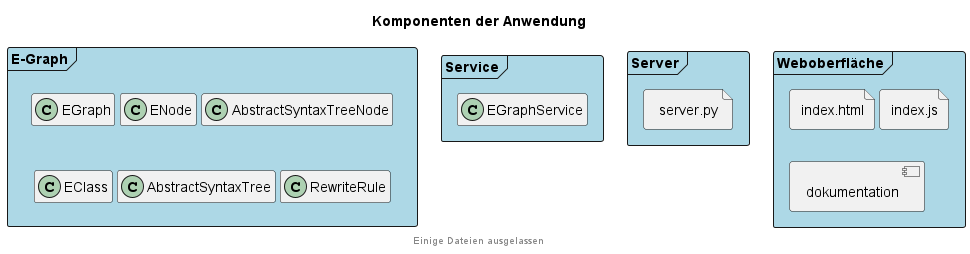
\includegraphics[scale=0.43]{utils/components.png}
        \caption{Architekturdiagramm der Anwendung}
        \label{fig:comps}
    \end{figure}
\end{frame}

\begin{frame}{Ablauf (1)}
    \begin{tcbitemize}[raster equal height=rows, raster columns=3, raster column skip = 1.5cm,
        raster every box/.style={size=small,valign=center,halign=center,colframe=white,colback=white}]
        \tcbitem {\Large $\left(\frac{x \cdot 2}{2} + x \cdot \frac{y - 3 + 3 + z \cdot 0}{x}\right)^2$ }
        \tcbitem \begin{tikzpicture}
            \draw[line width=10mm, -{Stealth[length=4mm, open, round]}, black, thick] (0,0) -- (2,0);
        \end{tikzpicture}
        \tcbitem {\Large $(x + y)^2$ }  
    \end{tcbitemize}\vspace{5mm}
\end{frame}

\begin{frame}{Ablauf (2): AST}
    \begin{figure}[H]
        \centering
        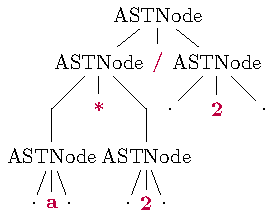
\includegraphics[scale=1.4]{utils/ast.pdf}
        \caption{\textbf{A}bstract \textbf{S}yntax \textbf{T}ree des Teilausdrucks $(x \cdot 2) / 2$}
        \label{fig:komponenten}
    \end{figure}
\end{frame}

\begin{frame}[fragile]{Ablauf (3): Add}
    %% add - Code
    \begin{columns}[c]
        \column{.7\textwidth}
        %\begin{lstlisting}[language=Python, escapechar=|, caption=Methoden der Klasse \textit{EGraph}, label={lst:methods1}]
\begin{minted}[fontsize=\small]{python}    
def add_node(self, ast_root_node): 
    # rekursiv Knoten des AST mit _add() zum E-Graph hinzufuegen 

def _add(self, enode): 
    enode = self._canonicalize(enode)
    if enode in self.h.keys(): 
        return self.h[enode]
    # weitere Faelle 
    else:
        eclass_id = self._new_singleton_eclass(enode)
        for child in enode.arguments:
            self.m[child].parents.add((enode, eclass_id)) 
        self.h[enode] = eclass_id
        return eclass_id
\end{minted}
                %\end{lstlisting}     
            \column{.3\textwidth}
            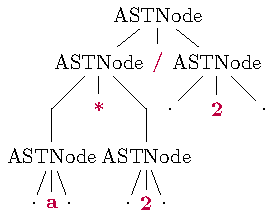
\includegraphics[scale=1]{utils/ast.pdf}
    \end{columns}
\end{frame}

\begin{frame}[fragile]{Ablauf (4): Apply}
    %% Apply - Code
\begin{minted}[fontsize=\small]{python}    
def apply_rules(rules, egraph):
    eclasses = egraph.get_eclasses()
    list_of_matches = []

    for rule in rules:
        for eclass_id, environment in egraph._ematch(eclasses, 
        rule.expr_lhs.root_node):
            list_of_matches.append((rule, eclass_id, environment))
    for rule, eclass_id, environment in list_of_matches:
        new_eclass_id = egraph._substitute(rule.expr_rhs.root_node, environment)
        egraph.merge(eclass_id, new_eclass_id)
        
    if egraph.pending:
        egraph.rebuild()
\end{minted}
\end{frame}

\begin{frame}[fragile]{Ablauf (5): Saturate}
    %% Eqsat - Code
\begin{minted}[fontsize=\small]{python}    
def equality_saturation(rules, eterm_id, egraph):
    best_term = ""
    old_term = best_term
    if not egraph.is_saturated:
        while True:
            best_term = _extract_term(eterm_id, egraph)
            if old_term == best_term:
                break
            old_term = best_term
            egraph = apply_rules(rules, egraph)     
\end{minted}
\end{frame}

\begin{frame}{Ablauf (5): Extract}
    \begin{columns}[c]
        \column{.5\textwidth}
            \textbf{Kostenfunktion}:
            \begin{itemize}
                \item Operatoren: \begin{itemize}
                    \item $+, -, \ll, \gg$: \textbf{1}
                    \item $*$: \textbf{2}
                    \item $/$: \textbf{3}
                \end{itemize}
                \item E-Node ohne Operatoren: \colorbox{green-400}{0}
                \item E-Node mit Operatoren: \colorbox{orange-400}{Operator + Kosten der Kinder}
                \item E-Class: \colorbox{blue-300}{Kind mit Minimum der Kosten}
            \end{itemize}
            
        \column{.5\textwidth}
            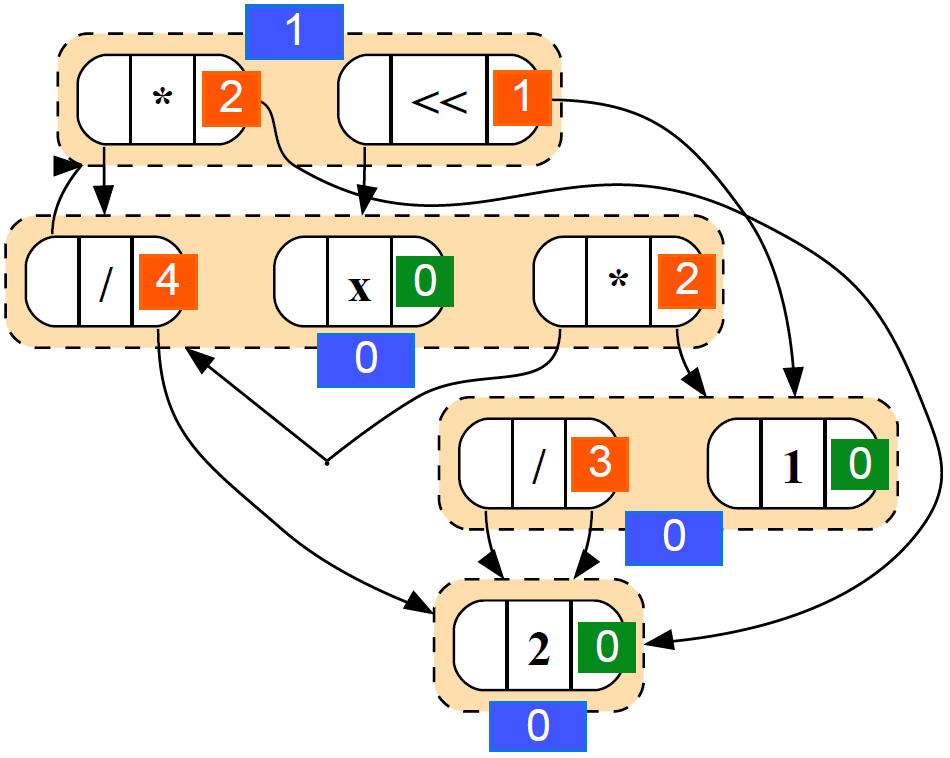
\includegraphics[scale=0.3]{utils/exp_egraph_colored.png}
    \end{columns}
\end{frame}

\begin{frame}{Ablauf (5): Extract}
    \begin{figure}[H]
        \centering
        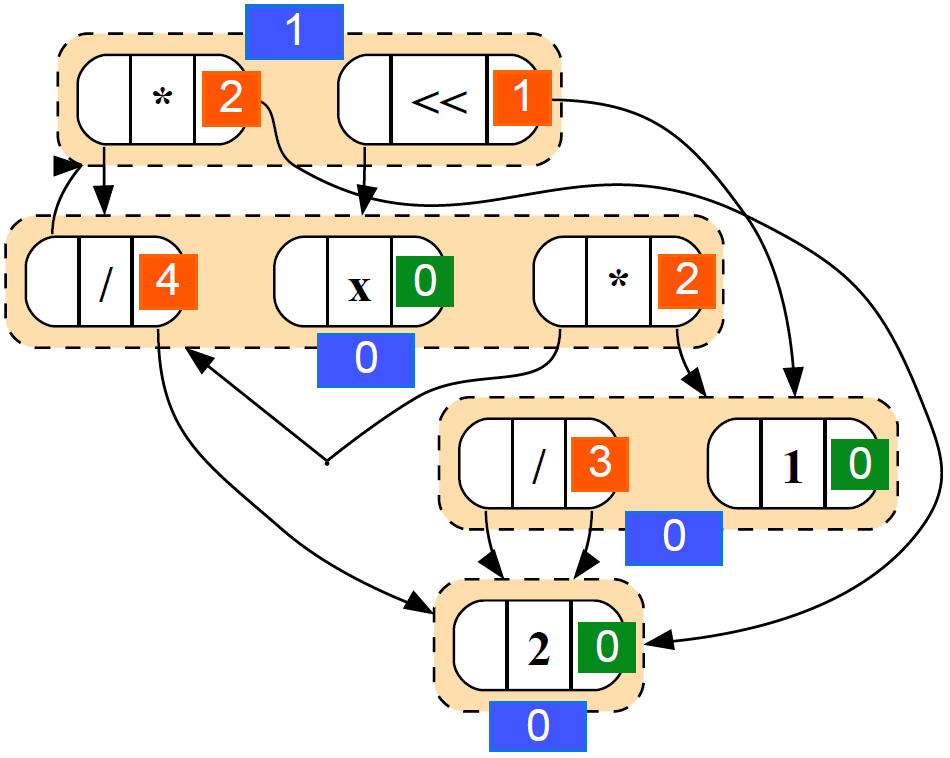
\includegraphics[scale=0.32]{utils/exp_egraph_colored.png}
        \caption{Kosten des Teilausdrucks $(x \cdot 2) / 2$}
        \label{fig:exp_egraph_costs}
    \end{figure}
\end{frame}